\chapter{MIP Heuristics}
Mixed Integer Program Heuristics can be applied in each MIP problem independently from the context. These do not consider the specific formulation of the TSP problem however they could have good applicability. In this report two MIP Heuristics will be discussed and compared with the  Metaheuristics

\section{Hard-fixing}
A simple idea to reduce the complexity of the problem is to get an initial solution like an incumbent, fix some active edges and resolve the subproblem with CPLEX. This is exactly the idea behind hard fix approach.\\
The implementation proposed is applied in sTSP problem, with the optimization of the general callback (\texttt{subtour\_callback\_general}).
The algorithm can be divided in step:
\begin{enumerate}
	\item calculate an initial solution: in our implementation this is done by CPLEX with \texttt{subtour\_callback\_general} and \texttt{CPX\_PARAM\_INTSOLLIM} set to 1. When the first incumbent is available,the optimization terminate and a solution is obtained.
	\item fix a percentage of edges (fixing rate $ f_r $): edges are fixed using \texttt{CPXchgbds()} method that change the upper and lower bound of the decision variables. The fixing percentage is an important parameter: fixing too much edges leads to a fast resolution of the subproblem however increase the risk of obtaining the same solution and fall in a loop. Fixing too low edges involves slower resolution. In the first iteration $ f_r = 0.9 $.
	\item CPLEX optimization with time limit: After the fixing phase, the problem is optimized with \texttt{CPX\_mipopt()} and a short time limit is set ($ = 50 $s).
	\item fixing rate update: after the last phase, if the returned solution is improved better than a fixed gap ($  good\_gap $), it is considered a good solution and the $ f_r $ is increased by a constant ($ incr\_f_r $) until a max ($ max\_f_r $) otherwise if the new solution is not increased enough (less than $ optimal\_gap $), $ f_r $ is decreased of a constant ($ decr\_f_r $) until a min ($ min\_f_r $). Note that $ good\_gap $ and $ optimal\_gap $ are expressed as fraction of the best lower bound.
	\item check end condition: if the time limit is reached, or $ f_r = 0.0 $ and the solution is not improved in the last iteration then the solution is returned. Note that in the second case, the best solution is found. In case that no ending condition is satisfy, the algorithm continue with point 3.
\end{enumerate}

The performance profile as shown in fig \ref{fig:Lsubtours_hardfixing_lightaverage_time}. Hard fixing has performance comparable with the exact model.

\begin{figure}[h]
	\centering
	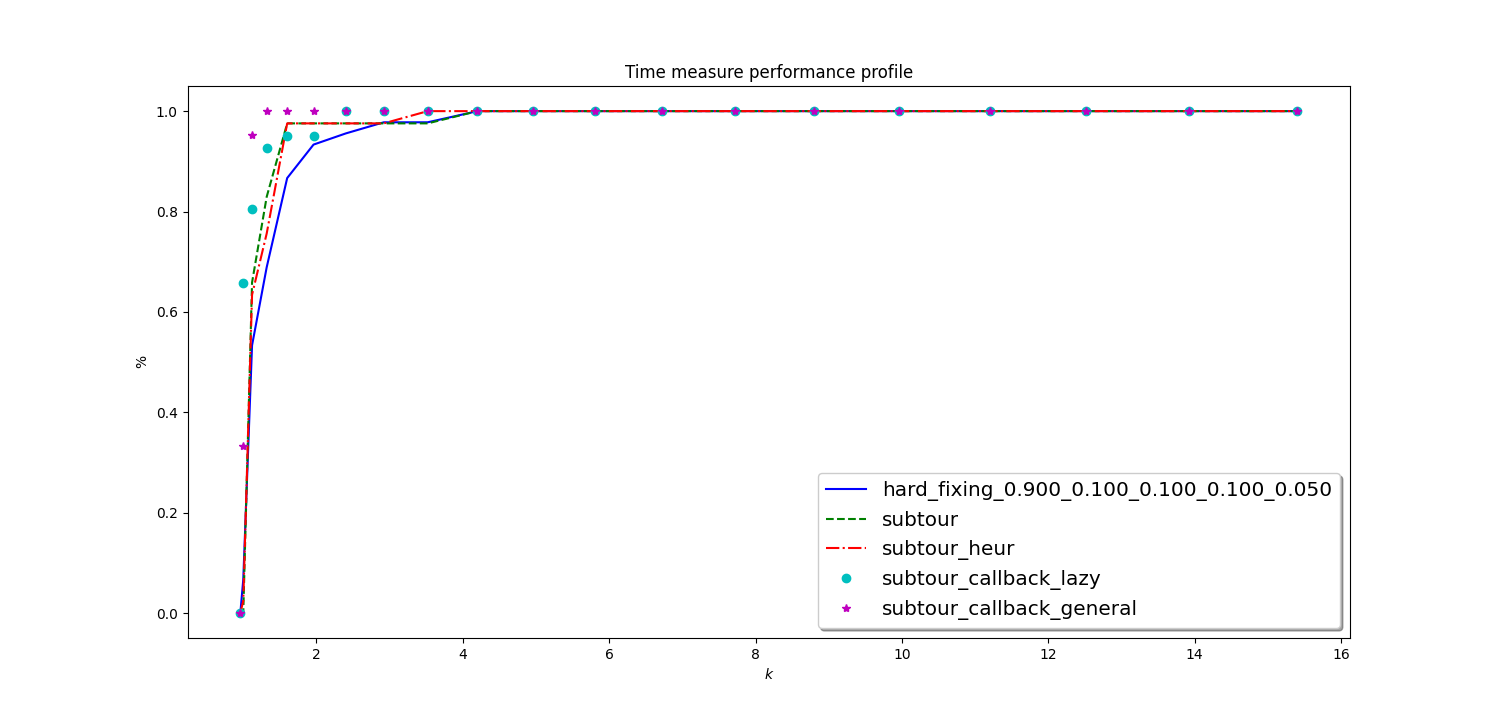
\includegraphics[width=\columnwidth]{../res/Lsubtours_hardfixing_lightaverage_time.png}
	\caption{Performance profile to compare subtours methods with \textit{hard\_fixing}. The name of \textit{hard\_fix} model contain in order: $ max\_f_r, incr_fr, decr\_f_r, good\_gap, optimal\_gap $. The test set is the composition of data\_light and data\_average.}
	\label{fig:Lsubtours_hardfixing_lightaverage_time}
\end{figure}


\section{Local-Branching}
The Hard Fixing method fix randomly a percentage of edges and optimize the problem, Local Branching (LB) instead let the MIP model to fix the same percentage of edges automatically and than optimize. Consider $ x^H $ as non optimal tour and $ \chi $ the fraction of edges to fix, LB add $ \sum_{ e\in E: x_e^H = 1 } x_e \ge \chi n $ to automatically fix the desired number of edges. 

\section{RINS}
\section{Feasibility Pump}
\section{Proximity Search}
\section{Polishing}
